\newpage
\section{Entwicklerhandbuch}

\begin{figure}[h]
	\centering
	
\includegraphics[scale=2.5]{03_Bedienungsanleitung/img/Logo_HFTl_App.png}
	\label{img:grafik-dummy}
\end{figure}

\begin{center}
	{\huge Entwicklerhandbuch}
\end{center}

\begin{center}
	{\huge -  HfTL-APP  -}
\end{center}

\begin{center}
	\textbf{{\large Stand: {\today}}}
\end{center}

\newpage
\tableofcontents
\newpage

\subsection{Allgemeines}
Dieses Dokument dient lediglich als Hilfswerkzeug zur (Weiter-)Entwicklung und Wartung der HfTL-App. In diesem Dokument ist der grobe Aufbau, sowie die wichtigsten verwendeten Funktion mitsamt zugehörigen Quelltext erklärt.
\\[1em]
Dieses Dokument ist keine Programmieranleitung.
\\[1em]
Es empfiehlt sich, gewisse Grundkenntnisse in objektorientierter Programmierung im Allgemeinen und  in JAVA, XML und AndroidStudio im Speziellen mitzubringen, um dieses Dokument effizient nutzen zu können.
\\[1em]
Standard-Methoden und Klassen sind nicht im Detail erklärt, da das den Rahmen dieses Dokuments sprengen würde. Für tiefer greifende Informationen wird die \href{http://developer.android.com/reference/packages.html}{Android-API} empfohlen.


\subsection{Verwendete Software}
\paragraph{AndroidStudio}
\ \\[1em]
AndroidStudio ist die Standard-Entwicklungsumgebung für Android. Es bietet bereits ein fertiges Gerüst für eine funktionsfähige App an. Das Programm bietet Klassenbibliotheken, Debugger und selbst ein Emulator mit dessen Hilfe Android-Endgeräte auf dem PC virtuell dargestellt werden können.\\
Das Programm kann kostenlos unter \href{https://developer.android.com/sdk/index.html}{developer.android.com} heruntergeladen werden.



\paragraph{GitHub}
\paragraph{Gimp}
\ \\[1em]
Gimp ist ein Open-Source Bildbearbeitungsprogramm. Es wurde in dem konkreten Fall genutzt, um Grafiken für die App zu erstellen.\\
Das Programm kann kostenlos auf der Seite des Herstellers  (\href{http://www.gimp.org/downloads/}{www.gimp.org}) herunter geladen werden.

\paragraph{Microsoft Office}

\subsection{Aufbau des Projekts}
\subsubsection{Manifest.XML}
Diese Datei ist für jede Android-App zwingend notwendig. Hier werden grundsätzliche Dinge definiert, z.B. Welche Berechtigung diese App benötigt und auf welche Hardware im laufenden Zustand zugegriffen werden muss.
\\\
Des Weiteren wird hier auch das package für den Javaquellcode definiert:\\\
\lstset{language=XML}
\begin{lstlisting}[caption={AndroidManifest.XML},label=package, frame=single]
<manifest xmlns:android="..." package="bkmi.de.hftl_app" >
\end{lstlisting}
Die Zugriffsberechtigungen sind wie folgt definiert:\\\

\begin{lstlisting}[caption={AndroidManifest.XML},label=permissions, frame=single]
<uses-permission android:name="android.permission.INTERNET" />
<uses-permission android:name="android.permission.ACCESS_NETWORK_STATE" />
<uses-permission android:name="android.permission.READ_PHONE_STATE" />
\end{lstlisting}
Bei der Installation der App wird der Nutzer entsprechend informiert, dass die App Zugriff auf die jeweiligen Funktionen des Endgerätes zugreift.
 \\\
In der manifest.xml ist ebenfalls eine Übersicht über die verwendeten Verzeichnisse und Komponenten hinterlegt, z.B. für die Activities.\\
Bei der HfTL-App ist der Verweis für die MainActivity (die Activity, mit der die App startet) für die NewsActivity gesetzt.
 \\\ 
Die folgenden Tags wurden bei der App nicht verwendet, sind aber theoretisch für Erweiterungen möglich:
\begin{lstlisting}[caption={Zugriffsbeispiel},label=perm-examble, frame=single]
<uses-feature android:name="android.hardware.camera" />
\end{lstlisting}
Das wäre ein Tag, um im laufenden Betrieb auf die Kamera des Telefons zuzugreifen.

\subsubsection{Ordnerstruktur}
\begin{description}
\item[Database]~\par
\begin{itemize}
\item beinhaltet die NotenDB.java – Inhalt ist der Connector und die Kernfunktionen um Inhalte der eigentlichen Datenbank zu aktualisieren und zu modifizieren
\item NotenTabelle.java – das ist die eigentliche Datenbank, bzw. die eigentliche Definition vom Aufbau der Datenbank
\end{itemize}

 
\item[Fragmente]~\par
\begin{itemize}
\item beinhaltet die Fragmente, die von den Activties verwendet werden.
\end{itemize}

\item[Service]~\par
\begin{itemize}
\item beinhaltet die Datei NotenService.java, die zum Erzeugen von Push-Nachrichten dient, sobald es in der Notenübersicht neue Noten für den jeweiligen Studenten gibt.
\end{itemize}

 
\item[Help]~\par
\begin{itemize}
\item beinhaltet diverse Hilfsunktionen, die unter anderem zum Ausführen von Threads dienen.
Ressourcen
\item unter /src/main/res befindet sich eine Ordnerstruktur, welche XML- und Bilddateien für verschiedenste Anwendungszwecke beinhaltet. Diese werden beim Kompilieren des Projekts in die Ressourcendatei R.java geschrieben. Über diese Datei, wird dann auf die Ressourcen zugegriffen
\end{itemize}

\item[Activities]~\par
\begin{itemize}
\item Hier werden allgemein Activities und deren Aufbau erläutert…
\item ...
\end{itemize}

 
\item[Fragmente]~\par
\begin{itemize}
\item Allgemeine Erklärung  zu Fragmenten
\item ...
\end{itemize}


\subsection{Activities}
\subsubsection{NewsActivity.java}
Klasse wird mit Fragment extended
NavigationDrawerFragment wird benötigt um die Interaktion mit Fragmenten zur Anzeige zu ermöglichen
Intent wird benötigt, um andere Activities neben der News Activity zu handlen.
mTitle ist der Titel des letztgeladenen Screens
 
\item[onCreate()]~\par
\begin{itemize}
\item Hier wird das Layout geladen, welches in der zugehörigen xml definiert wurde
\item Laden des mNavigationDrawerFragment, zum Abbilden des Menüs am linken Seitenrand
\item Laden des Layouts für das Fragment
 
Durch das Laden des Layouts für das mNavigationDrawerFragment (durch setUp) wird die Funktion onNavigationDrawerItemSelected gerufen, weil in der Layoutdefintion Item 1 der Listview ausgewählt wird.
\end{itemize}
 
\item[onNavigationDrawerItemSelected()]~\par
\begin{itemize}
\item Durch das Aufrufen der Funktion wird das eigentliche Fragment für den FragmentManager ausgewählt (durch die switch case Anweisung) und abschließend durch das commit aktiv geladen.
\end{itemize}

 
\item[onSectionAttached()]~\par
\begin{itemize}
\item Je nach Auswahl wird hier mTitle aktualisiert.
\end{itemize}

 
\item[restoreActionBar()]~\par
\begin{itemize}
\item Dient zum Aktualisieren der Titelleiste (durch setTitle und mTitle als Argument)
\end{itemize}

 
\item[onCreateOptionsMenu()]~\par
\begin{itemize}
\item Erstellt das Menü oben rechts (drei Punkte) und befüllt es mit den Daten aus der /res/menu/news.xml
\end{itemize}

 
\item[onOptionsItemSelected()]~\par
\begin{itemize}
\item Überprüft welches Element aus dem Menü ausgewählt wurde
\end{itemize}


\subsubsection{EinstellungsActivity.java}
 
\item[onCreate()]~\par
\begin{itemize}
\item Einbinden der “einstellung.xml“ (beinhaltet Definitionen für Stringvariablen, Listen und Checkboxen)
\item Setzen von Startwerten für shared, check und list
\item Ausführen von registerPreferenceListener()
\end{itemize}


\item[registerPreferenceListener()]~\par
\begin{itemize}
\item Es wird ein anonymer Listener erstellt, der auf Änderungen in der SharedPreference.xml reagiert
\item In der Methode onSharedPreferenceChanged(SharedPreferences prefs, String key) werden die Änderungen abgefangen
\item Listener wird am SharedPreferences Objekt  registriert
\end{itemize}

\item[testeBenutzerdaten()]~\par
\begin{itemize}
\item Funktion zum Überprüfen von Anmeldedaten
\item via TextSecure ts wird Ver- und Entschlüsselung gewährleistet
\end{itemize}


 
\item[keineBenutzerdaten()]~\par
\begin{itemize}
\item Funktion zum Ausgeben, dass die Anmeldeinformationen falsch eingegeben wurden
\end{itemize}

\subsection{NewsClickedActivity.java}
\lstset{language=JAVA}
\subsubsection{Allgemein}
Diese Activity wird geladen, sobald in der News-Übersicht (NewsActivity.java) ein Eintrag geöffnet wird. \\
Der Inhalt wird durch NewsResolver und dessen Funktion getDetailsStringArray in das String-Array s geladen.
\item[onCreate()]~\par
\begin{itemize}
\item Laden des in der zugehörigen xml definierten Layouts (activity\_ news\_ clicked.xml)
\item Einbinden der "Extras" (Übergebene Variablen)
\item Zuweisung der URL aus dem rufenden NewsFragment
\item Zuweisung der TextViews durch R.java
\begin{itemize}
\item Einbinden der verwendeten Schriftarten durch 
\begin{lstlisting}
 Typeface.java();
\end{lstlisting}
\item Zuweisung der Schriftarten an den jeweiligen TextView durch
\begin{lstlisting}
 setTypeface();
\end{lstlisting}
\item Aufruf des DetailHelpers durch 
\begin{lstlisting}
 new Detailhelper().execute();
\end{lstlisting}
\end{itemize}
\end{itemize}

\subsubsection{Klasse DetailHelper}
\item[onPreExecute()]~\par
\begin{itemize}
\item Anzeige eines ProgressDialogs, um den Anwender zu informieren
\end{itemize}

\item[onPostExecute()]~\par
\begin{itemize}
\item Ressourcen des ProcessDialogs werden freigegeben
\item Beschriftungen der Listboxen werden gesetzt.
\end{itemize}

\item[doInBackground()]~\par
\begin{itemize}
\item Neuinstanzierung eines NewsResolvers mit übergebener Url, um durch die Funktion getDetailsStringArray das Array s mit Daten zufüllen
\begin{lstlisting}
 s[0]=elements.get(0).child(1).text()+"\n";   //Ueberschrift
 s[1]=elements.get(0).child(2).text()+"\n";   //Subhead
 s[2]=elements.get(0).child(0).text();        //Zeit
 s[3]=elements.get(0).child(3).text();        //Text
\end{lstlisting}
\end{itemize}
\newpage
\subsection{Fragmente}
\subsubsection{NewsFragment}
Initialisierung erfolgt durch „NewInstance“, die aus der NewsActivity heraus gerufen wird. (siehe Funktionsaufruf -> onNavigationDrawerItemSelected)
Durch das .commit wird diese neue Instanz der Klasse dann geladen.
\paragraph{Überschriebene Funktionen:}
\ \\[1em]
\item[OnAttach()]~\par
\begin{itemize}
\item Verknüpfung des NewsFragments mit der MainActivity
\end{itemize}

\item[OnCreateView()]~\par
\begin{itemize}
\item Hier wird lediglich das Layout der View des Fragments geladen und angewendet
\end{itemize}

\item[onActivityCreated()]~\par
\begin{itemize}
\item es wird geprüft, ob es SavedInstances (bereitsgeladene Inhalte) gibt
\item wenn JA:
\begin{itemize}
\item die Informationen werden aus dem ARRAYSPEICHER geholt und angewandt
\end{itemize}
\item wenn NEIN:
\begin{itemize}
\item die Funktion „zeigeNews“ wird gerufen, welche die aktuellsten News vom Server lädt
\end{itemize}
\end{itemize}

 
\item[onStart()]~\par
\begin{itemize}
\item in dieser Funktion wird nur noch der Listener für den Aktualisierbutton mit der Schaltfläche verknüpft. Als onClick-Event wird dann lediglich die Funktion „zeigeNews“ gerufen.
\end{itemize}

 
\paragraph{standAllone-Funktionen}
\  \\[1em]
\item[isOnline()]~\par
\begin{itemize}
\item Diese Methode prüft durch einen Connectivity Manager, ob eine Verbindung zum Internet besteht
\end{itemize}

\item[zeigeNews()]~\par
\begin{itemize}
\item Zunächst wird durch „isOnline“ geprüft, ob eine aktive Netzverbindung besteht
\item wenn NEIN:
\begin{itemize}
\item Es wird ein Hinweis an den Nutzer ausgegeben
\end{itemize}
\item wenn JA: 
\begin{itemize}
\item Es wird eine Instanz der Klasse NewsHelper erstellt, welche dann als Hintergrund-Task ausgeführt wird, um ein Einfrieren der App zu verhindern.
\end{itemize}
\end{itemize}
\subsubsection{Klasse NewsHelper}
\begin{itemize}
\item Klasse mit asynchroner Task-Ausführung
\item Nach dem Aufruf der Methode \textit{zeigeNews} wird durch den Unterfunktionsaufruf \textit{.execute} zunächst die Funktion \textit{doInBackground} ausgeführt, wo eine neue Instanz des NewsResolvers erstellt wird.
\begin{lstlisting} 
private void zeigeNews(){
 NewsHelper nh = new NewsHelper();
 nh.execute();
}
\end{lstlisting}   
\item Durch \textit{getTermineStringArray} des NewsResolvers wird ein String-Array zurückgegeben.
\item Danach wird die Methode \textit{onPostExecute} gerufen.
\end{itemize}
\item[onListItemClick()]~\par
\begin{itemize}
\item Es wird ein intent verwendet um die \textit{NewsClickedActivity} zu starten, als "'Übergabeparameter"' wird \textit{putExtra} verwendet, im Falle der App die URL zu dem angeklickten Event.
\begin{lstlisting}
 intent = new Intent(getActivity(), NewsClickedActivity.class);
 intent.puExtra(TERMINDETAIL, newsResolver.getURLAsString(position));
 startActivity(intent);
\end{lstlisting}
\end{itemize}

\item[onPostExecute()]~\par
\begin{itemize}
\item  Überprüfung ob das Fragment noch aktiv ist
\begin{lstlisting}
if(getActivity()==null) return;
\end{lstlisting}
\item einbinden des \textit{CustomAdapterNews} in die ListView
\begin{lstlisting}
setListAdapter(new CustomAdapterNews(getActivity(), ...);
\end{lstlisting}
\end{itemize}

\subsubsection{NavigationDrawerFragment}
Dieses Fragment bildet das Menü auf dem linken Rand der App ab und aktiviert den Button mit dem man in die Einstellungen gelangt.

\item[onCreate()]~\par
In dieser Methode werden die Einstellungen der Activity übernommen und der Drawer ausgewählt. Außerdem wird geprüft ob eine gesicherte Instanz vorhanden ist, aus der dann das zuletzt ausgewählte Fragment ermittelt wird und über die Funktion \textit{selectItem()} aufgerufen wird. Falls keine gespeicherte Instanz existiert, wird die "'0"' (\textit{NewsFragment}) als Standardwert übergeben.
 
\item[onActivityCreated()]~\par
Hier wird das Menü für das aktuelle Fragment aktiviert indem an \textit{setHasOptionsMenu()} "'\textcolor{darkblue}{true}"' übergeben wird.
 
\item[onCreateView()]~\par
In dieser Funktion wird das Design für die Actionbar (als Listview) und die dazugehörigen Menüpunkte festgelegt. Zudem wird hier der ClickListener initialisiert, der dann den ausgewählten Eintrag an \textit{selectItem()} übergibt.

\item[isDrawerOpen()]~\par
Diese Methode prüft ob der Drawer bereits offen ist und liefert einen Wahrheitswert zurück.
 
\item[setUp()]~\par
Es werden hier folgende Einstellungen vorgenommen:
\begin{itemize}
\item Einstellungen zum Design
\item Aktivierung des HomeButtons und dessen Animation beim Draufklicken
\item Zusammenführung der \textit{ActionBar} und des \textit{NavigationDrawers}
\item weitere Einstellungen zum Drawer
\end{itemize}
Dann wird die Konfiguration in \textit{mDrawerToggle} abgespeichert

\item[selectItem()]~\par
Hier wird die Animation auf den angeklickten Menüpunkt ausgeführt.
Zudem wird der Drawer geschlossen und die Position des angeklickten Punktes an mCallbacks.onNavigationDrawerItemSelected() übergeben.
 
\item[onAttach()]~\par
Diese Methode setzt setzt den Zeiger mCallbacks auf die Activity.
 
\item[onDetach()]~\par
Hier wird der Zeiger \textit{mCallbacks} auf "'\textcolor{darkblue}{null}"' gesetzt.

\item[onSaveInstanceState()]~\par
Diese Funktion sichert die aktuelle Instanz.

\item[onConfigurationChanged()]~\par
Bei einer Änderung in den Einstellungen konfiguriert diese Methode \textit{mDrawerToggle} um.
 
\item[onCreateOptionsMenu()]~\par
Diese Funktion legt das Design, aus einer XML-Datei für das Menü Einstellungen, fest.
 
\item[onOptionsItemSelected()]~\par
Hier wird der Button, über den man zu den Einstellungen gelangt, aktiviert und mit dessen Klasse verknüpft.

\item[NavigationDrawerCallbacks()]~\par
Hier wird die ausgewählte Menüpunkt-ID an die Activity übergeben.

\subsubsection{Notenfragment}
\item[onCreateView()]~\par
\begin{itemize}
\item Laden des entsprechenden XML-Layouts \textit{fragment\_ noten.xml}
\item Laden und Zuweisung der Schriftart des TextViews für die Überschrift des Fragments
\end{itemize}

\item[onAttach()]~\par
\begin{itemize}
\item Aufruf der Datenbank, in der die Noteneinträge abgelegt werden
\end{itemize}

 
\item[onDetach()]~\par
\begin{itemize}
\item Schließen der Datenbank
\end{itemize}

 
\item[onStart()]~\par
Erstellen des Buttons zum Aktualisieren
Mittels \textit{OnClickListener} für den Button, wird über die Methode \textit{testeBenutzerdaten()} überprüft, ob die Benutzerdaten für QiS eingetragen wurden. Andernfalls erfolgt die Ausgabe mittels der Methode \textit{keineBenutzerdaten()}, dass diese nicht eingetragen wurden. Sofern die Benutzerdaten eingetragen wurden, und eine Onlineverbindung zu QiS besteht, werden die Noten erneut abgerufen. Ist keine Verbindung zu QiS vorhanden, wird der Nutzer mittels Toast-Benachrichtigung darüber informiert:\\
 
\includegraphics[scale=0.5]{05_Handbuch/img/Noten_Toast.png}

\item[getNoten()]~\par
Liest in der Notendatenbank alle Werte in der Spalte \textcolor{lila}{NOTENABFRAGE} aus und schreibt diese in das String-Array s, welches auch übergeben wird.
 
\item[getSemester()]~\par
Liest in der Notendatenbank alle Werte in der Spalte \textcolor{lila}{SEMESTERABFRAGE} aus und schreibt diese in ein String-Arrays, welches auch übergeben wird. Vor dem Schreiben des Arrays wird noch auf doppelte Werte geprüft. Sobald ein Wert in der Spalte doppelt ist, bleibt der Eintrag an der entsprechenden Position des String-Arrays \textcolor{darkblue}{NULL}. (Damit wird eine Auflistung der Noten und Fächer, aufgeschlüsselt nach Semester realisiert, siehe \textit{CustomAdapterNoten.java}.)
 
\item[getFach()]~\par
Liest in der Notendatenbank alle Werte in der Spalte \textcolor{lila}{FACHABFRAGE} aus und schreibt diese in das String-Array s, welches auch übergeben wird.

\item[getVersuche()]~\par
Liest in der Notendatenbank alle Werte in der Spalte \textcolor{lila}{VERSUCHABFRAGE} aus und schreibt diese in das String-Array s, welches auch übergeben wird.

\item[Hinweis:]~\par \textit{Die String-Arrays sind nur lokal in den jeweiligen Methoden definiert, weshalb diese - der Einfachheit halber - alle den Namen "'s"' erhielten. Tatsächlich werden hier vier unterschiedliche String-Arrays befüllt.}
 
\item[setzeListview()]~\par
Hier werden zunächst entsprechende String-Arrays durch die jeweiligen Methoden zur Abfrage in der Datenbank befüllt:
\begin{lstlisting}
notenList = getNoten();
semesterList = getSemester();
fachList = getFach();
versuchList = getVersuche();
\end{lstlisting}
Anschließend werden diese String-Arrays an den \textit{CustomAdapterNoten.java} übergeben. Damit wird eine individuelle Befüllung und Formatierung der Liste mit den ausgelesenen Werten aus der Datenbank realisiert.
 
\item[keineBenutzerdaten()]~\par
 
-- NotenHelper (Class)

\subsubsection{StundenplanFragment}

\item[newInstance()]~\par
Erstellt ein StundenplanFragment und "'steckt"' die aktive Position (aus dem Navigation Drawer) in das "'Bundle args"' welches als Argument im Fragment übergeben wird.
 
\item[onCreateView()]~\par
Laden des entsprechenden XML-Layouts fragment\_ noten.xml
Laden und Zuweisung der Schriftart für das TextView für die Überschrift des Fragments

\item[onViewCreated()]~\par
falls im “Stundenplanspeicher” Daten vorhanden sind werden diese geladen
Methode für das Dropdownmenü wird gerufen und Array für “events” erstellt
anonyme Listener für die Buttons werden erstellt

\item[erzeugeDropdown()]~\par
Dropdown aus xml einen Objekt zuweisen
Listener für Dropdown (als anonymer Listener) erzeugen und registieren
beim registieren wird die Methode onItemSelected aufgerufen und ein StundenplanHelper ausgeführt
Mittels eines “Calendar”, “Date” und zwei “SimpleDateFormat” wird das Dropdownmenü befüllt, indem die Daten in eine String-List eingefügt werden (list.add(temp))
Dropdown mit Liste verknüpfen
 
\item[keinStudiengang()]~\par
Prüft ob in den Einstellungen der Studiengang eingetragen wurde
falls nein -->Fehlermeldung

\item[erstelleStundenplan()]~\par
Erzeugt die Ausgabe des Stundenplans und fügt sie in den ListView ein
Falls keine Daten vorhanden sind wird “keine Daten” ausgegeben
 
-- StundenplanHelper (class)
 
\item[onPreExecute()]~\par
erzeugt ein Ladebalken
\item[onPostExecute]~\par
falls das Fragment noch aktiv ist wird die Methode erstelleStundenplan() gerufen
Ladebalken wird entfernt
 
\item[doInBackground]~\par
erzeugt ein StundenplanResolver
befüllt das “StundenplanEvents-Array Events“ mit Daten, durch die Methode “erzeugeStundenplan(String woche)” des StundenplanResolvers
falls ein Fehler auftritt wird ein Event erstellt in dem keine Daten sind


\newpage
\subsection{CustomAdapter} 
\subsubsection{Allgemein} 
Die CustomAdapter kommen da zum Einsatz, wo eine ListView genutzt und individuell befüllt werden muss. \\
Alle CustomAdapter entstehen durch Vererbung aus der Klasse BaseAdapter.java (\href{http://developer.android.com/reference/android/widget/BaseAdapter.html}{s. AndroidAPI}). Entsprechend sind einige Methoden vorgegeben, die initialisiert werden müssen (mit Rückgabewert), jedoch für die HfTL-App nicht (zwingend) von Bedeutung sind:
\begin{lstlisting}
   public int getCount()
   public Object getItem()
   public long getItemID()
\end{lstlisting}

Darüberhinaus ist der weitere Aufbau bei den drei verwendeten CustomAdaptern gleich. (Auf die jeweiligen Besonderheiten wird dann konkret im Abschnitt der jeweiligen CustomAdapter eingegangen):

Anfangs werden neue String-Arrays initialisiert, die mit den übergebenen Werten aus den Activities befüllt werden sollen.
\begin{lstlisting}
   String [] name;
\end{lstlisting}
Die abstrakte Klasse Context wird initialisiert und deklariert. (\href{http://developer.android.com/reference/android/content/Context.html}{s. AndroidAPI})
\begin{lstlisting}
   Context context;
\end{lstlisting}
Anschließend wird der Konstruktor der Klasse mit den jeweiligen übergebenen Parametern aufgerufen. \\ Welche Parameter genommen werden, hängt vom jeweiligen Aufruf des CustomAdapters in der entsprechenden Activity ab.
Nun werden die übergebenen Parameter den korrespondierenden Variablen zugeordnet.

\begin{lstlisting}
   public CustomAdapter (Activity nameActivity, String[] nameList){
    name = nameList;
    context = nameActivity;
   }
\end{lstlisting}


\item [class Holder]~\par
Dies ist ein Container mit TextViews
\begin{lstlisting}
   TextView tv_name;
\end{lstlisting}
Dieser Container wird dann als jeweilige Zeile in der ListView der zugehörigen Activity dargestellt.

\item [public View getView()]~\par
erstellt einen neuen Container 
\begin{lstlisting}
   Holder holder = new Holder;
\end{lstlisting}
erstellt eine View rowView
\begin{lstlisting}
   View rowView;
\end{lstlisting}
Das Layout der View und damit jeder Zeile in der ListView wird durch das Laden der entsprechenden XML namelist formatiert:
\begin{lstlisting}
   rowView = inflater.inflate(R.layout.name_list, null);
\end{lstlisting}
Die TextViews des Containers werden den entsprechenden TextViews in der XML zugeordnet:
\begin{lstlisting}
   holder.tv_name=(TextView)
   rowView.findViewbyId(R.id.namelist_name.xml);
\end{lstlisting}
Das TextView wird mit dem entsprechenden Wert des zugehörigen String-Arrays befüllt:
\begin{lstlisting}
   holder.tv_name.setText(name[position]);
\end{lstlisting}
Der nun befüllte Container wird nun als rowView übergeben.
\begin{lstlisting}
   return rowView;
\end{lstlisting}
\subsubsection{CustomAdapterNews.java} 
Dies ist der simpelste CustomAdapter der HfTL-App. Er wird verwendet um die News-Liste (also die Übersicht der News aus der HfTL-Homepage) zu formatieren.\\
Dabei werden drei String-Arrays (date, headline, content) in das zugehörige TextView der rowView übergeben. Der Inhalt dieser Arrays wird mittels der Klasse Newshelper, die wiederum die Methoden der Klasse NewsResolver aufruft, befüllt.
\subsubsection{CustomAdapterNoten.java}
Dieser CustomAdapter wird für die Befüllung der ListView des Notenfragments benutzt.\\
Hier werden vier String-Arrays (\textcolor{lila}{subject}, \textcolor{lila}{trys}, \textcolor{lila}{mark}, \textcolor{lila}{semester}) mit den Daten aus der Notendatenbank befüllt.\\
Entsprechend des Inhalts, werden die zugehörigen TextViews noch gesondert formatiert.\\
Ist der Inhalt an der Position des String-Arrays "'\textcolor{darkblue}{NULL}"', wird das zugehörige TextView auf "'\textcolor{lila}{GONE}"' gesetzt. So wird realisiert, dass mehrere Fächer unter dem selben Semester gelistet sind, ohne dass ein leeres (dunkelgraues) TextView erscheint.
\begin{lstlisting}
   if(semester[position]==null){
    holder.tv_semester.setVisibility(TextView.GONE);
   }
\end{lstlisting}
Auch für die jeweiligen Noten gibt es eine gesonderte Formatierung:
\begin{itemize}
\item Note schlechter als 5.0: \textcolor{magentat}{magenta}
\item Note schlechter als 3,4: \textcolor{gelbt}{gelb}
\item Note besser als 3,5: \textcolor{gruent}{gr"un}
\end{itemize}
\begin{lstlisting}
   if (mark[position].equals("5,0" ))
    holder.tv_mark.setTextColor
     (context.getResources().getColor(R.color.magenta));
   if (mark[position].equals("4,0" ) |
       mark[position].equals("3,9" ) |
       mark[position].equals("3,8" ) |
       mark[position].equals("3,7" ) |
       mark[position].equals("3,6" ) |
       mark[position].equals("3,5" ) )
            holder.tv_mark.setTextColor
             (context.getResources().getColor(R.color.gelb));
       else
            holder.tv_mark.setTextColor
             (context.getResources().getColor(R.color.gruen));
\end{lstlisting}

\subsubsection{CustomAdapterStundenplan}
Dieser CustomAdapter befüllt die ListView des StundenPlanfragments.\\
Hier werden fünf StringArrays(\textcolor{lila}{datum},\textcolor{lila}{fach},\textcolor{lila}{zeit},\textcolor{lila}{raum},\textcolor{lila}{kategorie}) übergeben, die zuvor mittels der Methode \textit{erstelleStundenplan()} des StundenplanFragments aus dem HTML-Code der QiS/HiS-Seite ausgelesen wurden.\\
Auch hier gibt es ein einige spezifische Formatierungen, abhängig vom übergebenen Inhalt.\\
Ist der Inhalt des StringArrays \textcolor{lila}{datum} an einer Stelle "'\textcolor{darkblue}{NULL}"', so wird die Sichtbarkeit des zugehörigen TextViews auf  "'\textcolor{lila}{GONE}"' gesetzt.\\
Analog zum \textit{CustomAdapterNoten} werden so die einzelnen Fächer unter dem selben Datum gelistet. Andernfalls würde über jedem Fach ein dunkelgraues TextView stehen.
\begin{lstlisting}
if(datum[position]!=null)
   holder.tv_date.setText(datum[position]);
else
   holder.tv_date.setVisibility(TextView.GONE);
\end{lstlisting}
Das StringArray \textcolor{lila}{kategorie} wird dazu verwendet, wichtige Ereignisse farblich kenntlich zu machen. Dabei wird nur der Inhalt an der jeweiligen Position des StringArrays geprüft und eine entsprechende (CI/CD-)Farbe für das Rechteck auf der rechten Seite verwendet:

\begin{itemize}
\item Prüfung: \textcolor{magentat}{magenta}
\item Praktikum: \textcolor{dunkelblaut}{dunkelblau}
\item Rest: \textcolor{grau01t}{grau01}
\end{itemize}
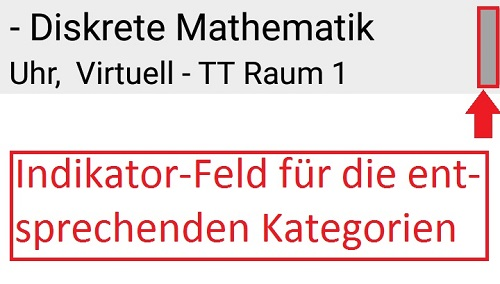
\includegraphics[scale=0.5]{05_Handbuch/img/kategorie.jpg}
\begin{lstlisting}
if (kategorie[position].equals("Pruefung"))
   holder.tv_category.setBackgroundColor
   (context.getRessources().getColor(R.color.magenta));
else if ((kategorie[position].equals("Praktikum"))
   holder.tv_category.setBackgroundColor
   (context.getRessources().getColor(R.color.dunkelblau));
else
    holder.tv_category.setBackgroundColor
   (context.getRessources().getColor(R.color.grau01));

\end{lstlisting}
\end{description} 